\documentclass[aps,prb, onecolumn,nofootinbib,citeautoscript,10pt]{revtex4-2}  
\synctex=1 


\usepackage{dcolumn}% Align table columns on decimal point
\usepackage{bm}% bold math
\usepackage{amsmath}
\usepackage{tabularx, graphicx}
\usepackage{epstopdf}
\usepackage{latexsym}
\usepackage{amssymb}
\usepackage{amsmath}
\usepackage{color, colortbl}
\usepackage{psfrag}
\usepackage{bbm}
\usepackage{titlesec}
\usepackage{dsfont}
\usepackage{slashed}
\usepackage{multirow}
\usepackage[tight]{subfigure}
\usepackage[papersize={8.5in,11in}]{geometry}

\usepackage{color}
\definecolor{darkblue}{rgb}{0.,0.,0.4}
\definecolor{darkred}{rgb}{0.5,0.,0.}
\definecolor{BlueViolet}{RGB}{138,43,226}
\definecolor{SkyBlue}{RGB}{30,144,255}
\definecolor{DarkGreen}{RGB}{0,100,0}
\usepackage[pdftex,colorlinks=true,linkcolor=darkblue,citecolor=blue,urlcolor=darkred]{hyperref}

\usepackage{physics}

\geometry{top=1.5cm, left= 1.5 cm, right= 1.5 cm, bottom=1.5cm}
\newcommand{\bs}[1]{\boldsymbol{#1}}



\def \nn{\nonumber \\}






%%%%%%%%%%%%%%%%%%%%%%%%%%%%%%%%%%%%%%%%%%%%%%%%%%%%%%%%%%%


\begin{document}


\title{Pseudo-Landau levels from strain-induced pseudomagnetic fields in tilted Dirac-cones}



\author{Sanskar Sharma}
\author{Ipsita Mandal}
\email{ipsita.mandal@snu.edu.in}

\affiliation{Department of Physics, Shiv Nadar Institution of Eminence (SNIoE), Gautam Buddha Nagar, Uttar Pradesh 201314, India}



\begin{abstract}
xxx
\end{abstract}


\maketitle

\tableofcontents

%%%%%%%%%%%%%%%%%%%%%%%%%%%%%%%%%%%%%%%%%%%%%%%%%%%%%%%%%%%%%%%%%%%%%%%%%%%%%%%%%%%%%


%%%%%%%%%%%%%%%%%%%%%%%%%%%%%%%%%%%%%%%%%%%%%%%%%%%%%%%%%%%%%%%%%%%%%%%%%%%%%%%%%%%%%
\section{Introduction}

The exceptionally novel electronic properties of graphene, a two-dimensional (2d) avatar of the allotropes of carbon, have contributed to exotic quantum-transport phenomena, which can be attributed to the emergent Dirac-cone dispersions. The Dirac-cones appear at the $K$ and $K^\prime $ points of the hexagonal Brillouin zone (BZ), when the Fermi level is set at the charge-neutral point of the system \cite{graphene-review}. BEDT-TTF- and BEDT-TSeF-based quasi-2d organic conductors under hydrostatic pressure, such as $\alpha$-(BEDT-TTF)$_2$I$_3$ and $\alpha$-(BEDT-TSeF)$_2$I$_3$ [where BEDT-TTF and BEDT-TSeF stand for bis(ethylenedithio)tetrathiafulvalene and bis(ethylene)dithiotetraselenafulvalene, respectively], also possess Dirac-cones like graphene \cite{organic-tilted-dirac, organic-dirac}. Usually, the pressure-dependent bandstructure exhibits a large anisotropy, e.g., tilted spectrum \cite{organic-tilted-dirac}. Electronic quasiparticles in the vicinity of a single cone can be described by an effective Weyl-like Hamiltonian in 2d. Using an effective tight-binding model on an anisotropic triangular lattice, with two sublattice sites (viz. A and B), one can show that the tilting of the Dirac-cones [cf. Fig.~\ref{figdis}] is caused by next-nearest-neighbour (nnn) hopping terms. A quinoid-type lattice-deformation can cause a tilt in the Dirac-cones of graphene as well. As argued in Ref.~\cite{tilted-goerbig}, a necessary requirement for the nnn hoppings to cause a tilt in the form of a linear-in-momentum term is that the Dirac-points (which are the locations of the Dirac-cones) be situated at points in the first BZ which do not coincide with the high-symmetry points (e.g., the corners $K$ and $K^\prime$ of the graphene lattice). In fact, if the Dirac-points (say, $D$ and $D^\prime $) coincide with the $K$ and $K^\prime$ points, then a quinoid-type graphene will have the nnn terms contributing only at the quadratic-in-momentum corrections.
%%%%%%%%%%%%%%%%%%%%%%%%%%%
Another point is that a tilt in the Dirac-cones of quinoid-type graphene will be less pronounced than that in the organic conductors, because the strength of the nnn terms is of the same order of magnitude as that of the nearest-neighbor (nn) hopping terms in the latter \cite{tilted-goerbig}. The reason behind this is the following: The locations of the Dirac-cones naturally deviate from high-symmetry crystallographic points in the organic compounds under pressure, leading to the nnn hopping terms becoming significant. One can capture the anisotropic features of the above systems via a generalized Weyl Hamiltonian that incorporates the tilt-parameters and any other anisotropy \cite{tilted-goerbig-plasmons, strained-dirac-franz, ips_tilted_dirac}. In particular, the nnn hopings also make the Fermi velocities ($v_x $ and $ v_y$) along the mututally-perpendicular momentum-axes to be unequal (i.e., $ v_x \neq v_y$).

Elastic strain has been used to manipulate the electronic properties of such 2d systems hosting Dirac-cones, opening up unprecedented opportunities for engineering quantum states through structural modifications \cite{neto-strain-graphene, strain-2d, graphene-strain-review, graphene-strain-geim, graphene-strain-terms, graphene-pseudo0, graphene-pseudo}. One of the remarkable outcome is the creation of strain-induced pseudomagnetic fields \cite{graphene-pseudo0, graphene-pseudo, strained-dirac-franz, complex-LL-strained-graphene}, which would cause pseudo-Landau levels (PLLs) to appear, analogous to the Landau-levels (LLs) appearing under the action of an actual magnetic field. The PLLs provide a route to realise the physics of Landau-level-quantization even under a zero magnetic field. The coupling of the fermionic quasiparticles with the mehcnaical strain is described using the pseudogauge field, $ \boldsymbol{\mathcal A}$, where the latter is generated by the lattice deformations. The pseudovector potential thus acts upon the charge carriers as if they were subjected to a magnetic field, $\boldsymbol{\mathcal B} = \nabla_{\boldsymbol r} \cross \boldsymbol{\mathcal A} $ \cite{pikulin16_chiral, ips_rahul_ph_strain, *ips-ruiz, ips-rsw-ph}. It is important to note that the nature of the coupling differs from that of an actual gauge field, the former being valley-dependent, where we refere to $D$ and $D^\prime $ as the two inequivalent valleys. The sign of the coupling switches for $D$ and $D^\prime $, as shown in Ref.~{strained-dirac-franz}. The situation is similar to the 3d versions embodied by a pair of conjugate Weyl nodes with opposite chiralities \cite{pikulin16_chiral}.

In this paper, we will study the nature of the PLLs for tilted Dirac-cones subjected to pseudomagnetic fields. Thus, our system possesses anisotropy from three ingredients: (i) $ v_x \neq v_y$; (ii) tilting; (iii) uniaxial strain. After deriving the nature of the discrete energy levels, we embark on deducing some basic features of linear repsonse in the form of electric conductivity.


%%%%%%%%%%%%%%%%%%%%%%%%%%
\begin{figure}[t]
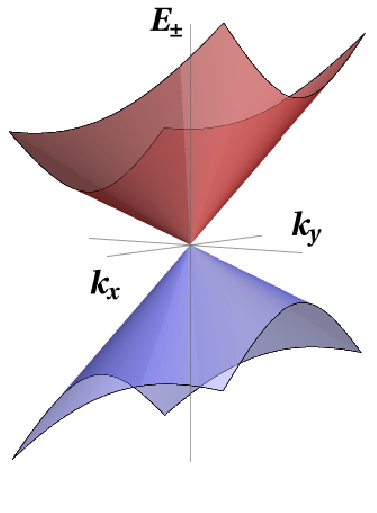
\includegraphics[width = 0.23 \textwidth]{disp}
\caption{\label{figdis}Energy bands for a tilted Dirac-cone.}
\end{figure}
%%%%%%%%%%%%%%%%%%%%%%%%%%%%%%%%
 

%%%%%%%%%%%%%%%%%%%%%%%%%%%%%%%%%%%%
\section{Model}
\label{secmodel}

%%%%%%%%%%%%%%%%%%%%%%%%%%%%%%%%%%%%%%%%%%%%

The minimal low-energy effective Hamiltonian of a single tilted Dirac-cone, at a valley indexd by $\xi $ (where $\xi =\pm$), is captured by~\cite{tilted-goerbig, ips_tilted_dirac}
\begin{align}
\label{eqham}
\mathcal{H}_0 =   \xi\, v_x\, k_x \,\sigma_x +    v_y \, k_y \,\sigma_y
+ \left ( \boldsymbol{v}_0 \cdot\boldsymbol{k} \right ) {\mathbb I}_{2\times 2} \,, \quad
%%%%%%%%%%%%%%%%%%%%%%%
\boldsymbol{v}_0 \equiv  
v_{0x} \,   {\boldsymbol{\hat x}} +  v_{0y} \,  {\boldsymbol{\hat y}}\,, \quad
v_{0x} \equiv   v_x\,\eta_x \, ,\quad
v_{0y} \equiv  v_y\,\eta_y \,,
\end{align}
where $\sigma_x $ and $\sigma_y $ denote the first two Pauli matrices. The velocities, $v_x$ and $v_y$, represent the components of the Fermi velocities along the $k_x$- and $k_y$-axes, respectively. Finally, the amount of tilt with respect to these two axes
are parametrised by $\eta_x$ and $\eta_y$, respectively. Clearly, the tilt introduces diagonal terms in the $2\times 2$ Hamiltonian, which did not exist in the untilted Dirac-cone case.
In the following, we will use the indices $\lbrace i, \, j \rbrace $ to label the component of a vector (or tensor) along the $
\lbrace i^{\rm th}, \, j^{\rm th} \rbrace$ Cartesian coordinate.


Here, we restrict ourselves to the cases when $ \eta <1$, where $\eta  \equiv \sqrt{ {\eta_x}^2 + {\eta_x}^2  }$, which implies that we are going to consider the type-I (or undertilted) phases, where the 1d Fermi surfaces at finite values of the chemical potential ($\mu$) are closed, i.e., ellipses. The energy eigenvalues of the two-band Hamiltonian are:
\begin{align}
E_{\pm} ({\boldsymbol k}) = (\boldsymbol{v}_0 \cdot \boldsymbol{k} )
 \pm \, \epsilon_k \,, \text{ where } 
\epsilon_k = \sqrt{ v^2_x \, k^2_x + v^2_y \, k^2_y } \,.
\end{align}


%%%%%%%%%%%%%%%%%%%%%%%%%%%
\subsection{Incorporating strain}

%The momentum-space Hamiltonian in the vicinity of a Dirac cone, containing only nn hoppings, can be expressed as
%\begin{align}
%& H_d = -\, t \sum_{\bs k} \sum \limits_{ \lbrace \bs M_\alpha \rbrace } \left[ 
%e^{ -\, i \, \bs k \cdot \bs M_\alpha} \, a_{\bs k}^\dagger \, b_{\bs k}
%+ 
%e^{  i \, \bs k \cdot \bs M_\alpha} \, b_{\bs k}^\dagger \, a_{\bs k}
%\right ], \quad \alpha \in \lbrace 1, \,2 ,\, 3 \rbrace \,,\nn
%%%%%%%%%%%%%
%& \bs M_1 = a_0 \, \bs{\hat y}\,, \quad \bs M_2 = - \frac{a_0}{2} \left(\sqrt 3 \,\bs{\hat x} + \bs{\hat y}\right),
%\quad \bs M_2 =  \frac{a_0}{2} \left(\sqrt 3 \,\bs{\hat x} - \bs{\hat y}\right).
%\end{align}
%Here, $a^\dagger _{\bs k}$ and $b ^\dagger _{\bs k}$  stand for the creation operators associated with the A and B sublattice degrees of freedom, respectively. The set $\lbrace \bs M_\alpha \rbrace$ denotes the nn-vectors for hoppings between the nn sublattices.



The real-space Hamiltonian in the vicinity of a Dirac cone, containing only nn hoppings, can be expressed as
\begin{align}
\label{eqnn}
& H_d = -\, t \sum_{\bs r_A} \sum \limits_{ \lbrace \bs M_\alpha \rbrace } \left[ 
a_{\bs r_A}^\dagger \, b_{\bs r_A + \bs M_\alpha} + b_{\bs r_A + \bs M_\alpha }^\dagger \, a_{\bs r}
\right ], \quad \alpha \in \lbrace 1, \,2 ,\, 3 \rbrace \,,\nn
%%%%%%%%%%%%
& \bs M_1 = a_0 \, \bs{\hat y}\,, \quad \bs M_2 = - \frac{a_0}{2} \left(\sqrt 3 \,\bs{\hat x} + \bs{\hat y}\right),
\quad \bs M_2 =  \frac{a_0}{2} \left(\sqrt 3 \,\bs{\hat x} - \bs{\hat y}\right),
\end{align}
where $a^\dagger_{\bs r}$ and $b ^\dagger _{\bs r}$ stand for the creation operators associated with the A and B sublattice sites, respectively, which are separated by the nn-distance $a_0$. The discrete coordinate-locations, $\bs r_A$ denote the A-sublattice sites and the set $\lbrace \bs M_\alpha \rbrace$ represents the nn-vectors for hoppings between the nn sublattices. We use the effective forms derived in Refs.~\cite{neto-strain-graphene, strained-dirac-franz} for a Dirac-cone subjected to uniaxial strain, which produces the pseudomagnetic fields that we want to analyse in this paper. In this procedure, the uniaxial strain pattern is incorporated in the system through a modulation of the nn hoppings into a  smooth function of the spatial coordinates. For the positions $\bs r_A $ and $\bs r_a + \bs M_\alpha $, the hopping amplitude is given the form of 
\begin{align}
t \rightarrow t_{\alpha}(\bs r_A) 
 = t_\alpha\, e^{-\gamma \,\Delta u_\alpha }
=  t  \left ( 1 -  \gamma_a \right)
 + \order{ \gamma _\alpha^2 } \,, \quad \gamma_\alpha \equiv \gamma\, \Delta u_\alpha, 
\end{align}
which depends on a displacement, $ \Delta u_{\alpha}$, along the three nn-bond directions. We assume the original displacement-field is $\bs u (\bs r) = u_x (\bs r)  \, \bs {\hat x} + u_y (\bs r) \, \bs {\hat y}$, such that $\bs u ({\bs r_A} + {}\bs M_\alpha) - \bs u (\bs r_A) = \Delta u_\alpha $, which we postulate to be of small magnitude (such that $\gamma_\alpha \ll 1 $).
Next, we are interested in a configuration of the strain tensor, $\varsigma_{ij}$, such that only its $\varsigma_{yy}$-component survives (i.e., $ \varsigma_{xx} = \varsigma_{xy} = \varsigma_{yx} = 0 $), which is purely $y$-dependent. Invoking the relation $\Delta u_{\alpha} = \sum_{i, j} \frac{ \left(M_\alpha \right)_i \left( M_\alpha\right)_j } {a_0}\,\varsigma_{ij}$, we deduce that
\begin{align}
\Delta u_1 = 4\, \Delta u_2 = 4 \, \Delta u_3 = a_0\, \varsigma_{yy}  (y)\,.
\end{align}



Although the authors in Ref.~\cite{strained-dirac-franz} derived the strain-induced terms for untilted isotropic Dirac-cones, initially located at the $K$ and $K^\prime $ corners of graphene's BZ, we assume that this applies also to the case of the tilted versions (shifted away from the high-symmetry points). This is justified because the Dirac-point and the $K$-point of the deformed
lattice do not coincide in general \cite{neto-strain-graphene}, which can be attributed to the fact that the applied strain not only affects the hoppings but also causes a distortion of the lattice itself. We just need to ensure that the strain to be applied in such a away that it affects mainly the off-diagonal terms arising from the nn hoppings. Therefore, in the vicinity of a Dirac-point hosting a tilted cone with anisotropic Fermi velocities as well, the applied strain modifies the continuum version of the low-energy Hamiltonian to \cite{strained-dirac-franz, complex-LL-strained-graphene}
%%%%%%%%%%%%%%
\begin{align}
\label{eqhtot}
& \mathcal H_\xi (k_x, y) = \left[ 
\left(v_x \, \eta_x \, k_x + v_y \,\eta_y\, k_y \right)  {\mathbb I}_{2\times 2} 
+ \mathcal{H}_s(y; k_x, k_y) \right ]\big \vert_{k_y \rightarrow -i\, \partial_y}
\,, \quad 
\mathcal{H}_s  = v_x \, d^\xi_x (\bs k)\,\sigma_x + v_y\,d^\xi_y (\bs k)\,\sigma_y  \,, \nn &
%%%%%%%%
\nn & d^\xi_x(\boldsymbol{k}) = \xi  \left (1 - \frac{ \tilde \gamma} {4}\right ) {k}_x 
+ \frac{ \tilde \gamma} {2\, a_0}  \,,
%%%%%%%%%
\quad  d^\xi_y(\boldsymbol{k}) =
\left (1 - \frac{3\, \tilde \gamma } {4} \right )  k_y 
+ \xi\, a_0\,\frac{ k_x \, k_y}{2} \left (1 - \frac{\tilde \gamma} {4}  \right ) ,
%%%%%%%%
\quad \tilde \gamma = \gamma\,a_0 \, \varsigma_{yy}\,.
\end{align}
%%%%%%%%%%%%%%%%%%%%%%%%%%%%%%%
Here, the index $\xi =\pm$ labels two inequivalent valleys. We observe that the $\varsigma_{yy}$ terms couples to the $k_x$ terms in a way such that the coupling of fermions with the effective pseudogauge-field component, $ \xi\, e \,  \mathcal{A}_x = \xi \, \tilde \gamma /(2\, a_0) = \xi\, \gamma \, \varsigma_{yy} / 2 $ (because, a gauge-field coupling is obtained by the substitution $k_x \rightarrow k_x - \text{charge } \times \mathcal{A}_x $). Thus, $ \mathcal{A}_x $ appears with opposite signs for $ D$ and $D^\prime$. In addition, we find that $\varsigma_{yy}$ also renormalises the values of the Fermi velocities. For a clearer visualization of the gauge-field coupling, remembering that $  
\tilde \gamma  = 2\, a_0 \,e \,  \mathcal{A}_x $, we rewrite the Hamiltonian with
%%%%%%%%%%%%%%%%%%%%%%%%%%
\begin{align}
 & d^\xi_x(\boldsymbol{k}) = \xi  \left (1 - \frac{ a_0 \,e \,  \mathcal{A}_x} {2}\right ) {k}_x 
+  \xi^2\,  e \,  \mathcal{A}_x  \,,
%%%%%%%%%
\quad d^\xi_y(\boldsymbol{k}) =
\left ( 1- 2\,a_0 \,e \,  \mathcal{A}_x  +  \frac{ \xi^2 \,a_0 \,e \,  \mathcal{A}_x} {2} 
\right )  k_y 
+  a_0\,\frac{ \xi\,k_x \, k_y}{2} \left (1 - \frac{ a_0 \,e \,  \mathcal{A}_x} {2}  \right ) \nn
%%%%%%%%%%%%%%%%%%%%%%%%%%%%%%%% next line 
%%%%%%%%%%%%%%%%%%%%%%%%%%%%%%%%%%
\Rightarrow & \; d^\xi_x(\boldsymbol{k}) = \xi  \,\Pi_x
  - \xi\,k_x  \frac{ a_0 \,e \,  \mathcal{A}_x} {2} \,,
%%%%%%%%%
\quad d^\xi_y(\boldsymbol{k}) =
\left ( 1- 2\,a_0 \,e \,  \mathcal{A}_x \right )  k_y  
+  \frac{ a_0\,\xi \, k_y} {2} \,\Pi_x \,,
\text{ where } \Pi_x =  k_x +  \xi \,  e \,  \mathcal{A}_x \,.
\end{align}
%%%%%%%%%%%%%
We find that a direct interpretation of the Hamiltonian as an analogy of actual LLs is a bit problematic because we have a mix of both $\Pi_x$ and $k_x $ terms. There has been the interpretation of the extra factors as a modulation of the Fermi velocities \cite{complex-LL-strained-graphene}, but we will take the point of view of solving for the energy levels of the resulting system and work out its eigenspectra, which we will call as the PLLs.


By taking $\mathcal{A}_x = -\, y\, {\mathcal B} $ (analogue of the Landau gauge), we can engineer $\bs{\mathcal B}= \nabla_{\bs r} \cross \bs{\mathcal A }$ to be directed perpendicular to the plane of the 2d lattice, which we call the negative $z$-direction. Therefore, we define
\begin{align}
 \varsigma_{yy} = \frac{2 \, b\, y} {\gamma} \,, \quad
b = e\, \mathcal B\,,
\end{align}
we generate $ \bs{\mathcal B} = -\,{\mathcal B} \, \bs{\hat z}$, which acts on the two valleys with opposite signs. Because of breaking the translation symmetry along the $y$-direction, $k_y $ is no longer a good quantum number, and we are forced to work in a hybrid spatial-momentum coordinates (viz. $y$ and $k_x$).


%%%%%%%%%%%%%%%%%%%%%%%%%%%%%%%%
\begin{figure*}[t!]
\centering
%\subfigure[]{\includegraphics[width= 0.6 \textwidth]{figPLL-notilt}}
\subfigure[]{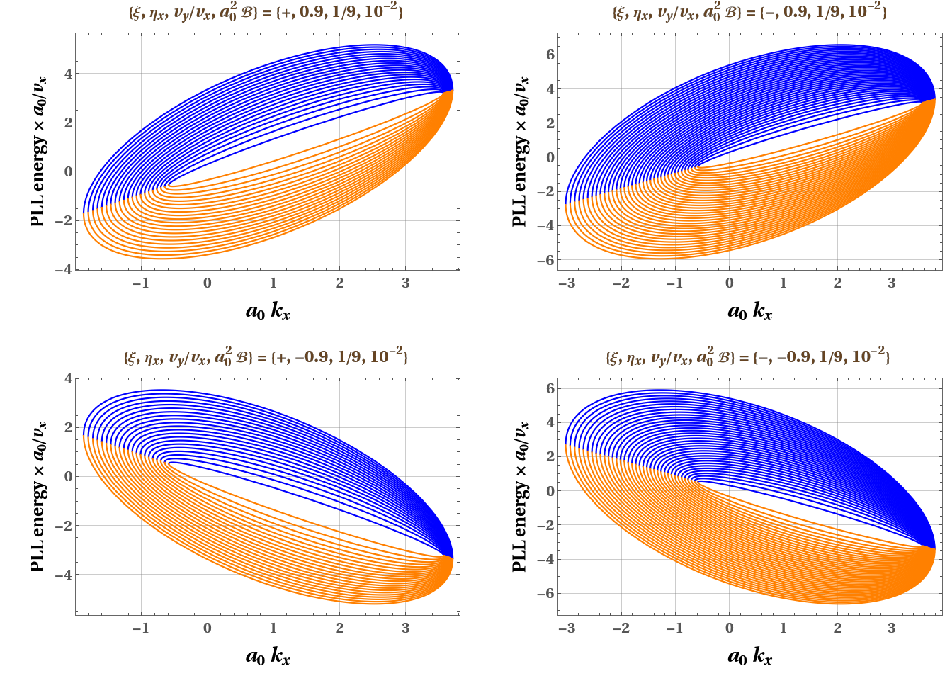
\includegraphics[width= 0.7 \textwidth]{figPLL}}
\subfigure[]{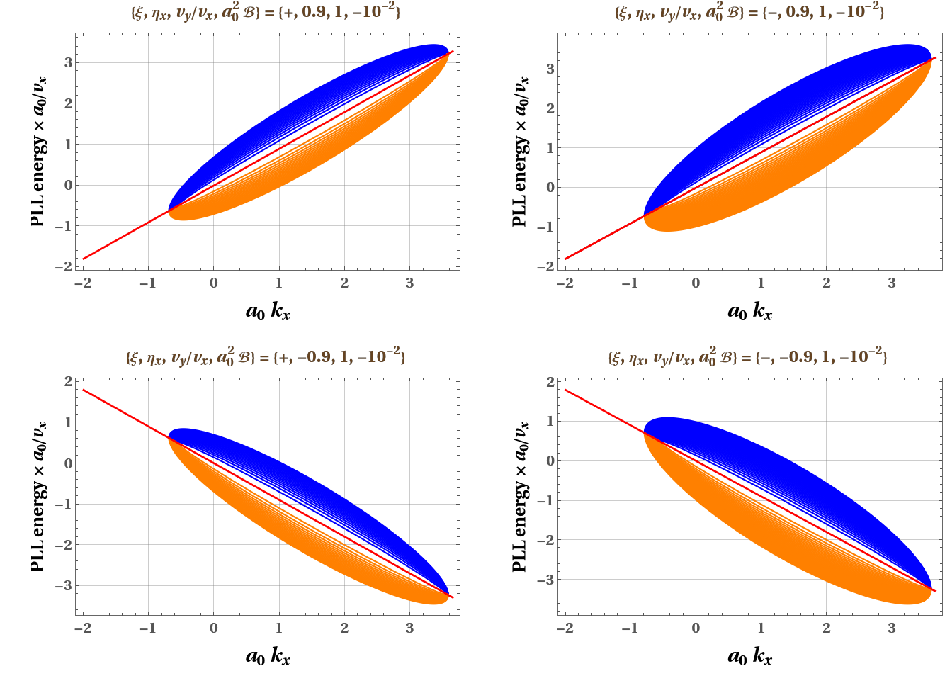
\includegraphics[width= 0.7 \textwidth]{figPLL2}}
\caption{Dispersion of the PLLs for some chosen parameters shown in the plot-labels. \label{fig:spectrum_B}}
\end{figure*}




%%%%%%%%%%%%%%%%%%%%%%%%%%%%%%%%
\subsection{Pseudo-Landau levels}
\label{secll}


To find the solution for the PLLs of the full Hamiltonian in Eq.~\eqref{eqhtot}, we need to solve for the eigenvalue equation,
\begin{align}
\mathcal{H}_{\xi} \,\Phi (k_x, y) = E \,\Phi (k_x, y)\,,\quad
\Phi^T (k_x, y) = \begin{bmatrix}
\phi_A (k_x, y) & \phi_B(k_x, y) 
\end{bmatrix} .
\end{align}
%%%%%%%%%%%%%
Since $k_x$ remains a good quantum number (because of unbroken translation symmetry along the $x$-direction), we work with the momentum-variable for the $x$-direction. The steps for solving the coupled differential equations involving the unknowns, $\phi_A$ and $\phi_B$, are detailed in Appendix~\ref{appdiff}.
Following those intermediate steps, we get the PLLs as
%%%%%%%%%%%%%%%%%%%
\begin{align}
\frac{E_{\xi, \text{si}}(n\, ; k_x) } {v_x} =  
\eta_x \,   k_x + \text{si} \, 
\sqrt{\tilde r_\xi^2 \, \left( |\zeta | \, n
+ \frac{e \, \mathcal B+|\zeta|}{2} \right)^2
+ \left (k_x \, \tilde r_\xi + s_{-\xi} \, s_\xi \right )
\left (2 \, |\zeta |\, n + e \, \mathcal B+|\zeta| \right )}  \,,
\text{ where } \tilde{r}_\xi = a_0 \, r_\xi \text{ and } \text{si} = \pm \,.
\end{align}
%%%%%%%%%%%%%%%%%%%%%%%%
We have labelled them by the integer-index $n$, momentum $k_x$, and band-index $\pm$ at the valley $\xi$. 
In the above, we have
\begin{align}
\tilde{r}_\xi = a_0 \, r_\xi \,, \quad \zeta =  e \, {\mathcal B} \, \frac{v_y}{v_x} \,, \quad
n \in \left\{ 0, \,1, \, 2,\cdots, 
\left\lfloor\frac{8 \,(2  + 3 \, \xi \,a_0\, k_x)}   { a_0^2\,|\zeta| \,(6 +\xi \,a_0\,  k_x)^2} \right\rfloor
\right\}.
\end{align} 
%%%%%%%%%%%
where $\left \lfloor  \Upsilon \right \rfloor$ denotes the greatest integer less than or equal to $\Upsilon$.
We get an upper-bound for the number of PLLs that depends on strain induced through the pseudo magnetic field in the system. For small $ |\mathcal V| $, the expression approximates to
%%%%%%%%%%%%%%%%%%%%%%%%%
\begin{align}
\frac{E_{\xi, \text{si}}(n\, ; k_x) } {v_x} \simeq    \eta_x \,   k_x 
+ \text{si}\, \sqrt{\left (k_x \, \tilde r_\xi + s_{-\xi} \, s_\xi \right )
\left (2 \, |\zeta |\, n + e \, \mathcal B+|\zeta| \right )} .
\end{align}
The plot for Landau Levels as given in Fig.~\ref{fig:spectrum_B} shows the dispersive landau levels , where the $\eta_x$ term causes the tilt in the landau levels as shown in figure.
We observe that the PLLs do not cut the origin, but they originate from the Dirac Points that are here shifted from the $k_x=0$ axis.  In other words, that there does not exist any zero-energy level in the system. Since $n\in \lbrace 0 \rbrace \cup \mathbb{Z}^+$, with a upper-bound of $
\left\lfloor\frac{8 \,(2  + 3 \, \xi \,a_0\, k_x)}   { a_0^2\,|\zeta| \,(6 +\xi \,a_0\,  k_x)^2} \right\rfloor$, we have a restrited number of PLLs. For positive values of $\eta_x$, it is possible for $E_{\xi, -}(n\, ; k_x)$
to take negative values as well. This happens when $ \eta_x \, a_0 \,  k_x  > \sqrt{\left (k_x \, \tilde r_\xi + s_{-\xi} \, s_\xi \right )
\left (2 \, |\zeta |\, n + e \, \mathcal B+|\zeta| \right )} $. Similarly, for $\eta_x<0$, we end up with negative values for $ E_{\xi, +}(n\, ; k_x)$ as well.




We represent the unique features of the PLLs by Fig.~\ref{fig:spectrum_B} for some representative parameter values.
The most intriguing nature that is revealed comprises the PLLs forming closed curves rather than dispersing out indefinitely as $ |k_x|$ is cranked up. No wonder that such closed curves are obtained for the tiltless casesas well. Furthermore, the range of PLL-curves are more expanded for the $D$-calley compared to the $D^\prime$-valley, showing that the system is not valley-symmetric. We find that the curves do not cut the origin, but instead are shifted due to the factor $\left (k_x \, \tilde r_\xi + s_{-\xi} \, s_\xi \right )$, which is the consequence of the fact that the Dirac points are no longer at the origin due to deformation in the system.

%%%%%%%%%%%%%%%%%%
\section{Conductivity using the Kubo formula}

%%%%%%%%%%%%%%%%%%%%%%%
\section{Conductivity using semiclassical Boltzmann formalism}

%%%%%%%%%%%%%%%%%%%%%%%
\begin{figure}[t!]
    \centering
    \includegraphics[width=0.443\textwidth]{cond}
    \includegraphics[width=0.443\textwidth]{condcomp}
    \caption{Plots for $\sigma_{xx}$ for $|b|=1$, while $h = e = k_B = 1$ . All plots are for Landau Levels ranging from $n=1$ to $n=9$, $\eta=0.7$ and $v_x=1$.The second plot compares the conductivity for different values of $\beta$, i.e., temperature.
\label{fig5}}
\end{figure}
%%%%%%%%%%%%%%%%%%%%%

The energy expression obtained in equation (25), can be used to plot the transport properties for the system. Using the Semi Classical Boltzmann Formalism, the expression for the conductivity tensor $\sigma_{ij}$ and the current density $J_i$ can be given by,\cite{park2017}
\begin{align}
\sigma_{ij}
=  e^2 \int \frac{d^2 k}{(2\pi)^2}
(-\frac{\partial f}{\partial \varepsilon})(\varepsilon)\,
v^i v^j \tau^j,
\
\end{align}
\begin{align}
J_{i}^{\xi, s}= \int \frac{dk}{2 \pi}[e f(E_n^s(k)\,v_{i}^s(k))],
\end{align}
where $v^{i,j}$ represent the group velocity in the $i^{th}$ and the $j^{th}$ direction, and $\tau$ is the relaxation time and $f$ is the Fermi-Dirac distribution function $f(\varepsilon)
= \frac{1}{e^{(\varepsilon - \mu)\beta} + 1}
$. Since the energy dispersion relation given above has only $k_x$ dependence, so only the group velocity along the x direction remains,and the remaining $v_y=v_z=0$. The group velocity along the $x$-direction can be given by $v_{x,n}^{\xi}(k_x)= \frac{\partial E_{\xi}(n\, ; k_x) }{\partial k_x}$, leads to
\begin{align}
{\color{red}
\frac{v_{x,n}^{\xi, \pm}(k_x)} {v_x}
=   \eta_x \pm \frac{a_0 \xi (e\,\mathcal   + |\zeta| + 2 |n \zeta|)}{2\sqrt{2} \sqrt{(2 + a_0 k_z \xi)(B e + |\zeta| + 2|n\zeta|)}} 
}
\end{align}
%%%%%%%%%%%%%%%
Due to the nonzero longitudinal group velocity $v_{x,n}^{\pm}$, while the transverse components satisfy $v_{y,n}^{\pm}=v_{z,n}^{\pm}=0$, the semiclassical Boltzmann approximation restricts the transport analysis to the longitudinal component $\sigma_{xx}$ of the conductivity tensor. Consequently, only the $J_x$ component of the valley current is relevant within this framework.
Fig. 4 presents the longitudinal conductivity $\sigma_{xx}$ calculated using this approach at finite temperature. Pronounced peaks in 
$\sigma_{xx}$ appear when the chemical potential coincides with the pseudo--Landau-level energies, reflecting the expected resonant response of a quantized spectrum. As the temperature is lowered, these peaks become sharper, whereas increasing temperature leads to significant broadening. This behavior is clearly illustrated in the second panel, where larger values of $\beta \, (\propto 1/T)$, such as $\beta = 200$, result in narrower and more well-resolved peaks, providing clear experimental signatures of pseudo--Landau-level formation.The plots are plotted within a very narrow range of $k_x$ varying, about the $k_x=0$ point, from $k_x= -0.043$ to $k_x=0.043$ keeping the singular point at $k_x=\pm 6$ out of the integration region.

%%%%%%%%%%%%%%%%%%%%%%%%%%%%%
\begin{figure}[t!]
    \centering
    \includegraphics[width=0.323\textwidth]{vallcurr}
    \includegraphics[width=0.323\textwidth]{vcurr comp}
    \includegraphics[width=0.323\textwidth]{betacurr}
    \caption{Plots for Valley current for $|b|=1$. All plots are for Landau Levels ranging from $n=1$ to $n=9$, $\eta=0.7$ and $v_x=1$.The first plot shows the total Valley current along $x$-direction, whereas the second shoes the plot for the same for different values of $B_s=|b|$, whereas the third for different values of $\beta = 1/T$.}
\end{figure}
%%%%%%%%%%%%%%%%%%%%%


The total bulk valley current show specific characterisitic when the chemical potential $\mu$ lies within a pseudo Landau Level, we expect pure valley currents in equilibrium in the bulk of the material. The strain-induced pseudo-magnetic field $|b|$ enters through the modified energy dispersion and creates valley dependent Landau like quantization. 
Fig[5], the first plot from the left illustrates the dependence of the longitudinal valley current $J_x$ on the chemical potential $\mu$ for a fixed pseudo-magnetic field. The staircase like structure of the curve arises from the quantization of
the electronic spectrum into dispersive pseudo Landau levels induced by the strain-generated gauge field. As $\mu$ increases, successive pseudo Landau levels become occupied, giving rise to discrete increases in $J_x$. Each plateau corresponds to a regime in which the number of occupied pseudo--Landau levels remains unchanged, while abrupt rises in the current occur when $\mu$ crosses a Landau-level energy. This step-like behavior provides a clear signature of quantized valley-resolved transport.The second plot shows show that increasing $|b|$ from $0.5$ to $1.5$ progressively suppresses the valley current due to the enhanced energy gaps and reduced state availability at a given chemical potential.The third plot depicts the dependence of the longitudinal valley current $J_x$ on the chemical potential $\mu$ at different temperatures, parameterized by $\beta = 1/k_B T$. The quantized staircase structure, arising from the sequential occupation of strain-induced pseudo-Landau levels, is acutely sensitive to thermal broadening. At low temperature ($\beta = 1000$), the Fermi-Dirac distribution is sharp, resulting in well-resolved, discrete steps in $J_x(\mu)$. As the temperature increases ($\beta$ decreases to $500$ and $10$), thermal smearing of the distribution progressively washes out these features, transforming the sharp staircase into a smooth, monotonic increase.


\section{Pseudoelectric field}

An interesting feature of inducing tilt in the system is that, the tilt induced in the system mimics the effect of the Isotropic, strained graphene case Ref.~\cite{strained-dirac-franz} for which the expression in the original frame reads like,
\begin{equation}
\frac{E_{\xi=1}(n;\,k_x)}{v_F}
\approx
-\beta k_x
+\frac{3}{2}\beta |bn|
+\operatorname{sgn}(n)(1-\beta^2)^{3/4}
\sqrt{|bn|(2+3k_x)}
\end{equation}
where, $\beta=\frac{\tilde{E}}{v_F \, \mathcal{B}}$, $\tilde{E}$ being the Electric field and $\mathcal{B}$ being the pseudo magnetic field. The $\beta$ term acts like a tilt similar to our case when $\eta_x \, \text{can be tuned to} \, \eta_x \propto \frac{1}{\mathcal{B}}$ giving the tilt effect to the system, and there can act as a pseudo electric field in the system.
\begin{align}
\frac{E_{\xi=1, \text{si}}(n\, ; k_x) } {v_x} \approx   \eta_x \,   k_x 
+ \text{si}\, \sqrt{\left (k_x \, \tilde r_\xi + s_{-\xi} \, s_\xi \right )
\left (2 \, |\zeta |\, n + e \, \mathcal B+|\zeta| \right )} .
\end{align}


%%%%%%%%%%%%%%%%%%%%%%%%%%%%%%%%%%%%%%%%%%%%%%%
\section{Discussions and future perspectives}
\label{secsum}

This results in a renormalized Fermi velocity and a modified density of states that profoundly influence the formation and characteristics of strain-induced quantum states.
Recent advances in strain engineering of two-dimensional materials have demonstrated remarkable control over electronic properties via lattice distortions. In particular, theoretical studies suggest that tailored strain in zigzag graphene nanoribbons can generate pseudomagnetic fields, giving rise to pseudo-Landau levels in the bulk and dispersive edge modes that reflect the interplay between strain, confinement, and boundary effects. \cite{strained-dirac-franz}. Such systems exhibit valley-helical transport, with counter-propagating valley currents at opposite edges, indicating a significant departure from traditional quantum Hall physics.
This work presents a comprehensive theoretical analysis of pseudo-Landau level formation in uniaxially strained anisotropic graphene. We examine how the pre-existing electronic anisotropy and tilt modify the formation, dispersion, and transport properties of PLLs. Our approach extends the established framework for strained graphene to account for the unique electronic features of anisotropic systems, providing fundamental insights into the interplay between structural modifications and external strain effects. The findings contribute significantly to the understanding of strain engineering in modified two-dimensional materials and open new pathways for controlling electronic properties through combined structural and mechanical manipulations.In this work, we investigate the formation of pseudo-Landau levels in uniaxially strained anisotropic graphene with tilted Dirac-cones, extending the framework of Ref.~\cite{strained-dirac-franz} to incorporate tilt effects arising from next-nearest-neighbor hopping. We derive analytical expressions for the dispersive energy spectrum by solving the coupled differential equations obtained from the low-energy Hamiltonian with both anisotropic Fermi velocities and tilt parameters. Our analysis reveals several key distinctions from the untilted case: (i) the energy dispersion exhibits qualitatively different scaling behavior with the pseudomagnetic field, leading to faster dispersion even at moderate momenta, (ii) the zero-energy Landau level is absent due to the modified quantization condition, and (iii) the tilt parameter introduces an overall energy shift and modifies the group velocities, directly impacting transport properties. We calculate the longitudinal conductivity within the semiclassical Boltzmann formalism and demonstrate characteristic quantum oscillations arising from resonant transport through discrete Landau levels. Our results provide insights into the interplay between structural modifications, strain engineering, and quantum transport in two-dimensional materials with broken rotational symmetry, with potential implications for valleytronic devices and strain-tunable quantum technologies.

In the future, we plan to incorporate another effect of a non-uniform strain, which is an emergent pseudoelectric field \cite{strained-dirac-franz}, which has been neglected in this work. We might have to resort to involved numerics to figure out the response of the system.


%%%%%%%%%%%%%%%%%
\appendix



%%%%%%%%%%%%%%%%%%%%%%%%%%
\section{Solving the differential equations}
\label{appdiff}


Starting with the Hamiltonian defined in Eq.~\eqref{eqhtot}, viz. 
\begin{align}
\label{eqhtotapp}
& \mathcal H_\xi (k_x, y) = \left[ 
\left( v_x \, \eta_x \, k_x + v_y \,\eta_y\, k_y \right)  {\mathbb I}_{2\times 2}
 + \mathcal{H}_s(y; k_x, k_y) \right ]\big \vert_{k_y \rightarrow -i\, \partial_y}
\,, \quad 
\mathcal{H}_s  =   d^\xi_x (\bs k)\,\sigma_x +  d^\xi_y (\bs k)\,\sigma_y  \,, \nn &
%%%%%%%%%%%
\frac{ d^\xi_x(\boldsymbol{k}) } {v_x} = \xi \, k_x + s_{-\xi} \, e \, {\mathcal B} \, y\,,
\quad
\frac {d^\xi_y(\boldsymbol{k})} {v_y} =  k_y  \left(s_\xi - r_\xi \, e \, {\mathcal B} \, y\, a_0
\right )  ,
%%%%%%%%%%%%%%
\quad s_\xi = 1 + \frac{\xi \, k_x\, a_0 } {2}\,, \quad
r_\xi = \frac{3}{2} + \frac{\xi \, k_x\, a_0 } {4} \,,
\end{align}
%%%%%%%%%%%%%%%%%%%
we follow the procedure detailed in Refs.~\cite{strained-dirac-franz, complex-LL-strained-graphene} to solve the eigenvalue equation, $\mathcal H_{\xi=1} (k_x, y) = E\, \Phi (y; k_x)$, by choosing the Dirac-point $D$. In this paper, we will consider tilt with respect to the $k_x$-axis only, setting $\eta_y = 0 $.



While dealing with the operators written in the $y$-space, we encounter terms of the form $i\, y\, \partial_y $, which are clearly not Hermiticised. One of the recipes of going from a classical operator (here, $ -i\, y\, \partial_y$) to its quantum version is symmetrisation, which we apply here (following Ref.~\cite{strained-dirac-franz}). Let us denote $y$ by $\hat y$ and $-i\, \partial_y$ by $\hat k_y$ to explicitly indicate that these are the position and momentum operators along the $y$-direction, projected into the position-space representation. Then we must replace any occurrence of $ -i\, y \,\partial_y $ by
$$ \frac{\hat{y} \,\hat{k}_y}{2}  +   \frac{\ \hat{k}_y \hat{y} }{2} = \hat{y} \,\hat{k}_y + \frac{1}{2} \,.$$
Going back to our original notation, we just replace $ -i\, y \,\partial_y $ by $-i\left ( y\,\partial_y + 1/2 \right)$ in the final expressions. After eliminating $\phi_A$ using the two equations arising from the two spinor components and shifting the $y$-coordinate as $ y\rightarrow y + 
\frac{s_+}{r_+ \,a_0\,  e\, {\mathcal B}}$, the final equation for $\phi_B$ turns out to be
%%%%%%%%%%%%%%%%%%%%%%%%%%%%
\begin{align}
\label{eqdiffea}
& \left[(s_{-}\,e \, {\mathcal B}\,y)^2 + \frac{s_{-} \,e \, {\mathcal B}}{\tilde{r}}(2\,k_x\,\tilde{r}+2\,s_{-}\,s_+
-e \, {\mathcal B}\,\tilde{r}^2)\,y+\frac{\Delta}{\tilde{r}^2}-\frac{\zeta^2\,\tilde{r}^2}{4} \right] \, \phi_B 
-2 \,y \, \zeta^2 \, \tilde{r}^2 \, \phi_B'-y^2 \, \zeta^2 \, \tilde{r}^2 \, \phi_B^{\prime \prime} = 0\,,
%%%%%%%%%%%%
\nn & \tilde{r} = a_0 \, r_+ \,, \quad \zeta =  e \, {\mathcal B} \, \frac{v_y}{v_x} \,, \quad
\epsilon = a_0 \, \left( \frac{E}{v_x}- \eta_x \, k_x \right), \quad
\Delta = (k_x \, \tilde r+ s_{-} \, s_+ )^2-\tilde r^2 \, \epsilon^2 \,.
\end{align}
%%%%%%%%%%%%%%%%%%%
%For nonzero $\eta_y$, there are imaginary terms which necessitate taking $\phi_B $ to be complex, which we parametrise as 
%$ \phi_B(y) = A_\phi (y) + i \,B_\phi (y)$. Taking the real and imaginary parts, we arrive at
%%%%%%%%%%%%%%%%%%
%\begin{align}
%& \left[(p_+ \,b\,y)^2+\frac{ p_+ \, b\, y} {r_+ } \left (2\,k_x\,r_+ +2 \, p_+ \, s-b\,r_+^2 \right )
%+\frac{\Delta}{r_+^2}-\frac{b^2\,r_+^2}{4}
%-\frac{1}{4}   \right] A_\phi 
%-\left (2 \,y \, b^2\, r_+^2 + 2\,y \right ) \partial_y A_\phi
%\nn & -\, y^2 \left (b^2 \,r_+^2+1 \right ) \partial^2_y A_\phi 
%+ \epsilon \,\eta_y \, B_\phi  
%+ 2\,y \,\epsilon \,\eta_y\, \partial_y B_\phi = 0 \,, \nn
%%%%%%%%%%%%%%%%%%%%%%
%& \left[( p_+ \,  b\, y)^2 + \frac{ p_+ \,  b\, y } {r_+ } \left (2 \,k_x\,r_+ + 2\, p_+ \, s-b\,r_+^2 \right )
%+\frac{\Delta}{r_+^2}-\frac{b^2 \,r_+^2}{4}-\frac{1}{4}\right]B_\phi
%-\left (2 \,y \,b^2 \,r_+^2 + 2\,y \right ) \partial_y B_\phi
%-y^2 \left (b^2 \,r_+^2+1  \right ) \partial^2_y B_\phi \nn &
%-\epsilon\, \eta_y \, A - 2\,y \,\epsilon\, \eta_y\,\partial_y A_\phi =0 \,.
%\end{align}
%%%%%%%%%%%%%%%%%%%
%These are coupled equations in $A_\phi$ and $B_\phi$, which make analytical solutions unfeasible. Hence, we consider the simpler case with $\eta_y = 0$ and solve for real $\phi_ B $ , as considered in Refs.~\cite{tilted-goerbig-plasmons, strained-dirac-franz}.
%%%%%%%%%%%%%%%%%%%%%%%%%%
The above form is in the form of a Strum-Liuouville (SSL) problem, viz. $\partial_y \left[ \mathcal P (y)\,\partial_y \phi_B \right ] - \, {\mathcal Q} (y)\,\phi_B = -\,\lambda\, {\mathcal W}(y)\,\phi_B $. In fact, it is a singular SSL scenario because the interval $(-\infty, 0]$ (or, $ [0, \infty)$) infinite and ${\mathcal P} (y) = 0$ at the boundary $y= 0$. Next, we perform an asymptotic analysis of the system at $y\rightarrow0$ and $ |y| \rightarrow \infty$ \cite{strained-dirac-franz}:
%%%%%%%%%%%%%%%%%%%
\begin{itemize}
\item For $y\rightarrow0$, the leading-order terms reduce to
\begin{align}
\left[\frac{\Delta}{\tilde{r}^2}-\frac{\zeta^2\,\tilde{r}^2}{4} \right] \, \phi_B 
-2 \,y \, \zeta^2 \, \tilde{r}^2  \, \phi_B'- \zeta^2 \, \tilde{r}^2 \,y^2 \, \phi_B^{\prime \prime}=0 \,,
\end{align}
which has solutions going as $\phi_B \sim y^{-\frac{1}{2}\pm{\frac{\sqrt{\Delta}}{\tilde{r}^2 \, |\zeta|}}} $. The $y=0$ regime represents one with regular singularity. The only physically-admissible solution is  $ \phi_B \sim y^{-\frac{1}{2}+{\frac{\sqrt{\Delta}}{\tilde{r}^2 \, |\zeta|}}} $, since the other one diverges. 

\item For $ |y| \rightarrow\infty$, we need to solve for
\begin{align}
\left (s_{-}\,e \, {\mathcal B}\,y \right )^2  \phi_B -y^2 \,\zeta^2 \, \tilde{r}^2 \, \phi_B^{\prime \prime}=0 \, ,
\end{align}
which has the solution of the form, $ y \sim \exp \left [ {\pm \, e\, |{\mathcal B}|  \,s_{-} \, y} /(\tilde r \, \zeta) \right ] $. 
Each solution diverges either at $ y = \infty$ or $y=-\infty $ and, hence, none is physically admissible along the entire $y$-axis. These points are therefore irregular singularities.

\end{itemize}
%%%%%%%%%%%%%%%%%%%%%
Knowing the forms of the asymptotic expressions, we now take the ansatz \cite{strained-dirac-franz} (suppressing the explicit $k_x$-dependence),
% \\\textcolor{red}{here}
\begin{align}
\phi_B (y) = e^{-\tilde y/2} \, 
y^{-\frac{1}{2}+{\frac{\sqrt{\Delta}}{\tilde{r}^2 \, |\zeta|}}} \,  u(y) \,,\quad
%%%%%%%%%%%%%%
\tilde y = -\, \frac{ 2\, v_x \, \text{sgn} (\mathcal B) \,s_{-}\, y} { v_y \,\tilde r } \,.
\end{align}
%%%%%%%%%%%%%%% 
Changing variables from $y$ to $\tilde y $ and defining $\tilde u(\tilde y) = u(y)$,
we end up with a confluent hypergeometric differential equation for $\tilde u(\tilde y)$, away from the singularity [considering the interval to be either $(-\infty, 0]$ or $ [0, \infty)$], which can be expressed as
\begin{align}
& {\tilde y}\, \partial^2_{\tilde y} \tilde u (\tilde y)
+ (\Gamma- \tilde y)\, \partial_{\tilde y} \tilde u({\tilde y})-\alpha \,\tilde u({\tilde y}) = 0\,, \quad
\alpha = \frac{\tilde r^2 \, (e \, {\mathcal B}+|\zeta|)+ 2 \, (\sqrt{\Delta}-s_{-} \, s_+ -k_x \, \tilde r)} 
{2 \, |\zeta| \, \tilde r^2} \,, \quad
%%%%%%%%%%%%%%%%%%%%
\Gamma = 1+ \frac{2 \,\sqrt{\Delta }}{\tilde  r^2 \, |\zeta|}\, .
\end{align}
%%%%%%%%%%%%%%%%%%%%%%
It turns out that the regular solutions involve the Kummer’s function, $\mathcal M (\alpha, \Gamma, \tilde y)$, where $\alpha = - n $ (taking $n \in 0 \cup {\mathbb{Z}}^+ $) is a non-positive integer but $\Gamma $ is not. Then, we have the condition that
\begin{align}
-\,n = \frac{\tilde r^2 \, (e \, {\mathcal B}+|\zeta|)+ 2 \, (\sqrt{\Delta}-s_{-} \, s_+ -k_x \, \tilde r)} 
{2 \, |\zeta| \, \tilde r^2} 
%%%%%%%%%%%%
\Rightarrow
\sqrt{\Delta}=-\tilde r^2 \, |\zeta |\, n+k_x \, \tilde r-\frac{\tilde r^2}{2}
(e \, \mathcal B+ |\zeta|)+s_{-} \, s_+ \,.
\end{align}
%%%%%%%%%%%%%%%%%%%%%%%%%%%%%
Using the relation $ \Delta = (k_x \, \tilde r+s_{-} \, s_+ )^2-\tilde r^2 \, \epsilon^2 $, it leads to
\begin{align}
\epsilon^2 = \tilde r^2 \, \left( |\zeta |\, n + \frac{e \, \mathcal B+ |\zeta|}{2} \right)^2
+ \left (k_x \, \tilde r+s_{-} \, s_+ \right ) \left (2 \, |\zeta |\, n + e \, \mathcal B+|\zeta| \right),
%%%%%%%%%%%%%
\quad \mathcal M (-n, \Gamma, \tilde y) = {\mathcal L}^{\Gamma-1}_{n}(\tilde y)\,,
\end{align}
where ${\mathcal L}^\ell_{n} (\tilde y )$ is the Generalized (or, alternatively, Associated) Laguerre polynomial with $ n \in 0 \cup {\mathbb Z}^+$. Imposing the requisite physical condition that $\epsilon^2 \geq 0 $, we obtain an upper bound for $n$ as $ 
\left\lfloor\frac{8 \,(2  + 3 \, \xi \,a_0\, k_x)}   { a_0^2\,|\zeta| \,(6 +\xi \,a_0\,  k_x)^2} \right\rfloor  $. The symbol $\left \lfloor  \Upsilon \right \rfloor$ denotes the greatest integer less than or equal to $\Upsilon$. The final solution is obtained as \cite{strained-dirac-franz}
\begin{align}
& \phi_B (k_x, y+ y^+_{\rm sg}) \, \Theta \left[ \text{sgn}(\mathcal B ) \left(- y\right)  \right],\,
\text{ where }\nn
%%%%%%%%%%%%%%%%%%%%
 &\phi_B (k_x, y) = e^{\frac{  v_x \, \text{sgn} (\mathcal B) \,s_{-\xi}\, y} { v_y \, r_+\, a_0 }} \, 
y^{-\frac{1}{2}+{\frac{ v_x \,\sqrt{\Delta}}{ r_\xi^2\, a_0^2\, e  \, v_y  \left |{\mathcal B}  \right |}}} \, 
{\mathcal L}^{\Gamma-1}_{n}(\tilde y)\,, 
%%%%%%%%%%%%%
 \quad  y^+_{\rm sg} = \frac{s_+ } {r_+ \,a_0\,  e\, {\mathcal B}}\,,\quad
\tilde y = -\, \frac{ 2\, v_x \, \text{sgn} (\mathcal B) \,s_{-}\; y} 
{ v_y \,r_+\, a_0 }\,.
\end{align}
%%%%%%%%%%%%%%%%%%%%%%%%%
Clearly, the full wavefunction does not diverge at the irregular singularity, as it is cut-off by the Heaviside-theta function and it goes to zero before reaching that singular point.



The same process can be repeated for the valley with $\xi =- $. Using $E= \frac{v_x} {a_0} \left[  \eta_x \,   k_x + \epsilon   \right ]$, we finally get the PLLs as
%%%%%%%%%%%%%%%%%%%
\begin{align}
\frac{E_{\xi, \text{si}}(n\, ; k_x) } {v_x} =  
\eta_x \,   k_x + \text{si} \,
\sqrt{\tilde r_\xi^2 \, \left( |\zeta | \, n
+ \frac{e \, \mathcal B+|\zeta|}{2} \right)^2
+ \left (k_x \, \tilde r_\xi + s_{-\xi} \, s_\xi \right )
\left (2 \, |\zeta |\, n + e \, \mathcal B+|\zeta| \right )}  \,,
\text{ where } \tilde{r}_\xi = a_0 \, r_\xi \text{ and } \text{si} =\pm\,.
\end{align}
%%%%%%%%%%%%%%%%%%%%%%%%
We have labelled them by the integer-index $n$, momentum $k_x$, and band-index $\pm$ at the valley $\xi$. The valley-dependent wavefunction, for the $n^{\rm th}$ PLL, is captured by
\begin{align}
& \phi_B^{\xi,n, \text{si}} (k_x, y+ y^\xi_{\rm sg}) \, \Theta \left[ \text{sgn}(\mathcal B ) \left(- y\right)  \right],\,
\quad
%%%%%%%%%%%%%%%%%%%%
 \phi_B^{\xi, n, \text{si}} (k_x, y) = e^{\frac{ v_x \, \text{sgn} (\mathcal B) \,s_{- \xi}\, y} { v_y \, r_\xi\, a_0 }} \, 
y^{-\frac{1}{2}+{\frac{ v_x \,\sqrt{\Delta}}{ r_\xi^2\, a_0^2\, e  \, v_y  \left |{\mathcal B}  \right |}}} \, 
{\mathcal L}^{\Gamma-1}_{n}(\tilde y)\,, 
\quad  \Gamma = 1+ \frac{2 \,\sqrt{\Delta }}{\tilde  r_\xi^2 \, |\zeta|} \,,\nn
%%%%%%%%%%%%%
& \quad  y^\xi_{\rm sg} = \frac{s_\xi } {r_\xi \,a_0\,  e\, {\mathcal B}}\,,\quad
\tilde y = -\, \frac{ 2\, v_x \, \text{sgn} (\mathcal B) \,s_{-\xi}\, y} 
{ v_y \,r_\xi \, a_0 }\,, \quad
%%%%%%%%%%%%%%%%%%%
\sqrt{\Delta}=-{\tilde r}_\xi^2 \, |\zeta |\, n + k_x \, {\tilde r}_\xi -\frac{\tilde r_\xi^2}{2}
(e \, \mathcal B + |\zeta|)+s_{\xi} \, s_{-\xi} \,.
\end{align}
%%%%%%%%%%%%%%%%%%%%%%%%%
We also show below the explicit expression for the upper component of the $n^{\rm th}$-PLL's eigenspinor, $ \Phi^{\xi, n, \text{si}} (k_x, y) = \begin{bmatrix}
\phi_A^{\xi, n, \text{si}}  (k_x, y) && \phi_B^{\xi, n, \text{si}}  (k_x, y)  \end{bmatrix}^T $:
%%%%%%%%%%%%%%%%%%%%%%%%%%%%
\begin{align}
\label{eqphia}
& \phi_A^{\xi, n, \text{si}} (k_x, y)  =  \frac{1}{v_x} \frac{
e^{\frac{2v_x \,\mathrm{sgn}(\mathcal{B})\, s_{-\xi}\, y}{v_y\, r_\xi\, a_0}}
\, y^{-\frac{3}{2} + 
\frac{v_x \sqrt{\Delta}}{r_{\xi}^2\, a_0^2\, e\, v_y\, \left|\mathcal{B}\right|}}
\left[
{\mathcal{F}}_1^\xi\,\mathcal{L}_{n}^{\Gamma-1}(\tilde{y})
-
{\mathcal{F}}_2^\xi \,\mathcal{L}_{n-1}^{\Gamma-1}(\tilde{y})\right]}
{ \frac{E_{\xi, \text{si}}(n\, ; k_x)} {v_x} - \eta_x \,   k_x }\,,
%%%%%%%%%%%%%%%%%%%%%%%%
\nn & {\mathcal{F}}_1^\xi   = 8 \, v_x  \, F_1^\xi  \, F_2^\xi + 8 \,  r_\xi
\left [ 4 \,v_y|\mathcal{B}|\,r_\xi\,F_3^\xi 
+ 8  \, \mathcal{B} \, v_x \,  y\,F_4^\xi  \right ],\quad
%%%%%%%%%%%%%%%%%%%%%%%%%%
{\mathcal{F}}_2^\xi  = 256\, v_x\, y\, |\mathcal{B}|\, r_\xi
\left[a_0 \,\mathcal{B} \,y \,r_\xi + v_y \left (s_\xi-2 \right )\right]
(s_\xi-2)\, \text{sgn}(\mathcal{B})\,,
\end{align}
where
\begin{align}
F_1^\xi  &=  2 \, \mathcal{B}  \, r_\xi^2 + a_0^2 \,  k_x^2 \left (1 - \xi \right )
-6 \, a_0  \, k_x - 4\,, \quad
%%%%%%%%%%%%%%%%%%
F_2^\xi  = 4 \, a_0 \, \mathcal{B} \, y  \, r_\xi + 4 \, v_y\left (s_\xi-2 \right ), \nn
%%%%%%%%%%%%%%%%%%%%
F_3^\xi  &= 4\,v_y \left (n+1 \right ) \left (s_\xi-2 \right ) 
+k_x  \,  \xi \,y \left[ a_0^3  \, \mathcal{B}\,(n+1)-4 \, v_x\right]
+6 \, a_0^2 \, \mathcal{B}\,(n+1)\,y\,, \nn
%%%%%%%%%%%%%%%%%%%
F_4^\xi  & = y\, r_\xi \left(4 \,a_0\,\mathcal{B}\,s_\xi-8\,a_0 \, \mathcal{B}
+ a_0 \,\xi\, v_y-2\, v_y \right)
+ 4\,v_y\left(s_{-\xi} \, s_\xi-1\right).
\end{align}

%%%%%%%%%%%%%%%%%%%%%%%%%
\section{Kubo formula}

For finding the linear response in the form of the longitudinal magneto-optical conductivity for the $x$-direction, we will use
the Kubo formala~\cite{ashby-carbotte},
\begin{align}
\label{eqkubo}
% taken from eqn 11 of B 111, 075125 (2025)
%%%%%%%%%%%%%%%%%%%%%%%%%%%%%%%%%%%%%%%%%%%%%%%
\sigma^\xi_{xx}(\omega) &= -\frac{i} {\mathcal S} \, \sum_{n,n^\prime} \, \sum_{\text{si},\text{si}^\prime}
\int \frac{dy\, dk_x}{2\pi} \left[ \frac{f_{\xi, n ,\text{si}} (k_x) - f_{\xi, n^\prime ,\text{si}^\prime}(k_x)} 
	{E_{\xi,\text{si}} (n; k_x) - E_{\xi, \text{si}^\prime}(n^\prime; k_x)} \right ] 
\frac{ \mathcal{M}^{n, n^\prime}_{\text{si}, \text{si}^\prime} (k_x, y)}
	{\omega + E_{\xi, \text{si}}(n;k_x) - E_{\xi, \text{si}^\prime} (n^\prime; k_x) + i \, \delta} \,,\nn
%%%%%%%%%%%%%%
 \mathcal{M}^{n, n^\prime}_{\text{si}, \text{si}^\prime} & =  
\left [ \left(\Phi^{\xi, n, \text{si}}\right)^\dagger \,J_x \, \Phi^{\xi, n^\prime, \text{si}^\prime} \right ]
 \left [ \left(\Phi^{\xi, n^\prime, \text{si}^\prime }\right)^\dagger \,J_x \, \Phi^{\xi, n, \text{si}} \right ],
 %%%%%%%%%
\nn \frac{J_x} {e} & =  \frac{\partial {\mathcal H}_{\xi} (k_x, y) }{\partial k_x} 
=  v_x \,\eta _x\, \mathbb{I}_{2\times 2}
-\frac{\xi \, v_x  } {2} \left(a_0 \,e \,{\mathcal B} \, y-2\right)  \sigma _x
-\frac{a_0\, \xi \, k_y \,v_y }{4}  \left(a_0\, e\, {\mathcal B} \, y-2\right) \sigma_y. 
\end{align}
%%%%%%%%%%%
where $\mathcal S $ is the sample's area along the $x$-axis, $\omega $ denotes the frequency of the absorbed/emitted photon and $\delta$ denotes the impurity scattering rate. For the sake of simplicity, we have assumed that all the PLLs have the same value of $\delta $.

%%%%%%%%%%%%%%%%%%%%%%%%%%%%%%%%%%%%%
\section{Semiclassical Boltzmann equations}

For the semiclassical Boltzmann formalism applied to this system, the valley-resolved current density is derived from the general expression

\begin{align}
J_{i,n}^s(\mu)= \int \frac{dk}{2 \pi}[e f(E_n^s(k)v_{n,i}^s(k))],
\end{align}
 In our case, the strain-induced pseudomagnetic field quantizes the spectrum into a set of dispersive PLLs, $E_{n}^{s}(k)$, which are valley-dependent due to the opposite sign of the effective gauge potential. Therefore, the total valley current $J_{i}(\mu)$ is obtained by performing the integration for each discrete Landau level, followed by a summation over both the Landau level index $n$ and the valley index $s$:
%%%%%%%%%%%%%%%%%
\begin{align}
\label{eq:J_total}
J_{i}(\mu) = \sum_{s=\pm} \sum_{n} J_{i,n}^{s}(\mu) = e \sum_{s=\pm} \sum_{n} \int \frac{dk}{2\pi} \, f\big(E_{n}^{s}(k)\big) \, v_{n,i}^{s}(k).
\end{align}
The resulting total valley current, $J_{i}(\mu)$, can be finite even when the individual valley contributions $J_{i}^{+}(\mu)$ and $J_{i}^{-}(\mu)$ are symmetric in magnitude, as the pseudomagnetic field generates valley dependent group velocities that are odd under $s \leftrightarrow -s$. Since our energy expression has only $v_x$ dependence, therefore this leads to the $J_x$ component of the current density. For same reasons, the transport analysis is restricted to the longitudinal component of the conductivity tensor Consequently, the relevant quantity is the longitudinal conductivity $\sigma_{xx}$, given by,
\begin{align}
\sigma_{xx}^s(\mu)
=  -i\, e^2 \sum_{n} \int \frac{d k_x}{(2\pi)}
(-\frac{\partial f (E_n^s(k_x)-\mu)}{\partial(E_n^s(k_x))})\,
v_{n,x}^2(k_x) \tau_x(k_x),
\
\end{align}
where $\tau_x \propto v_{n,i}^2(k) $ for a given valley index s.
\label{secb}

%%%%%%%%%%%%%%%%%
\label{secsum}

%%%%%%%%%%%%%%%%%%%%%%%%%%

\bibliography{ref_ll}

 
\end{document}
